% !TEX program = lualatex
\documentclass[12pt,a4paper]{article}
\usepackage{graphicx}
\usepackage{fontspec}
\setmonofont{Latin Modern Mono}
\usepackage{xcolor}
\usepackage{listings}
\usepackage{geometry}
\usepackage{fancyhdr}
\usepackage{hyperref}
\usepackage{booktabs} 
\usepackage{float}    
\usepackage{amsmath}

% =======================================================
%  USER CONFIGURATION (EDIT VARIABLES HERE)
% =======================================================
\newcommand{\labNo}{Lab 4}
\newcommand{\labTopic}{Integrity Constraints, Sorting, Subqueries, and Data Filtering}
\newcommand{\courseCode}{CSE 4308}
\newcommand{\courseTitleShort}{DBMS Lab}
\newcommand{\courseTitleLong}{DATABASE MANAGEMENT SYSTEMS LAB}
\newcommand{\instructorName}{Samnun Azfar, Jr. Lecturer, CSE\\ Samia Nawsheen, Jr. Lecturer, CSE}
\newcommand{\academicYear}{AY25-26}
% =======================================================

\geometry{margin=1in}

% -
% Header and Footer Configuration
% -
\pagestyle{fancy}
\fancyhf{}
\lhead{\labNo}                        % Uses variable
\rhead{\courseCode: \courseTitleShort} % Uses variables

% Centered footer with page number
\cfoot{\thepage}
% Ensure header/footer width matches text block
\setlength{\headwidth}{\textwidth}

% -
% Code Listing Style
% -
\definecolor{codegreen}{rgb}{0,0.6,0}
\definecolor{codegray}{rgb}{0.5,0.5,0.5}
\definecolor{codepurple}{rgb}{0.58,0,0.82}
\definecolor{backcolour}{rgb}{0.95,0.95,0.92}

\lstdefinestyle{mystyle}{
    backgroundcolor=\color{backcolour},
    commentstyle=\color{codegreen},
    keywordstyle=\color{magenta},
    numberstyle=\tiny\color{codegray},
    stringstyle=\color{codepurple},
    basicstyle=\ttfamily\footnotesize,
    breaklines=true,
    captionpos=b,
    keepspaces=true,
    numbers=left,
    numbersep=5pt,
    tabsize=2,
    frame=single,
    numbers=none,
    columns=fullflexible,
    showspaces=false,
    showstringspaces=false,
    showtabs=false,
    language=SQL
}

\lstset{style=mystyle}

% Images: found next to this file (local compile_labs.sh) or via the
% lab folder when compiled from the project root (Overleaf).
\graphicspath{{lab_04_integrity_constraints_sorting_subqueries/}}

\begin{document}

% --
% TITLE PAGE
% --
\begin{titlepage}
    \centering
    \vspace*{2\baselineskip}

    \rule{14cm}{2pt}\vspace*{-0.8\baselineskip}\vspace*{1.5pt}
    \rule{14cm}{0.5pt}\vspace{2\baselineskip}

    {\Huge\bfseries\scshape \labNo\par} % Uses variable
    \vspace{3mm}
    {\Large \labTopic} % Uses variable
    \vspace{3mm}

    \rule{14cm}{0.5pt}\vspace*{-0.7\baselineskip}\vspace{2.5pt}
    \rule{14cm}{2pt}

    \vspace{2\baselineskip}

    {\Large\bfseries \courseCode\par} % Uses variable
    \vspace{1\baselineskip}
    {\large \courseTitleLong\par} % Uses variable

    \vfill
    {\normalsize Prepared by:\\ \instructorName\par} % Uses variable
    {\normalsize Academic Year: \academicYear\par} % Uses variable
\end{titlepage}

\newpage
\tableofcontents
\newpage
\section*{Lab Workflow}



\textit{Repeat this subsection for every single lab.}

\begin{enumerate}
\item Connect to the internet by running nmtui in terminal, add a dsl connection, then go back and activate that dsl connection. Make sure that your net id is not being used in any other pc or router, if you face any issue, use any other net id from your friends which is not being used.

\item Download all the files posted in the google classroom.

\item Disconnect from the \textbf{dsl} connection via nmtui, connect to the ethernet/wired connection via nmtui. If no such connection exists, create an \textbf{ethernet} connection  and then activate.

    \item \textbf{Create Your Role and Database}

Inside the PostgreSQL shell, create your own role (user) and database.

1. In the Linux terminal:
\begin{lstlisting}[language=bash]
psql
\end{lstlisting}

Expected prompt:
\begin{lstlisting}
cse=#
\end{lstlisting}

2. Create Your Role and Database

Copy and run the following commands inside PostgreSQL:
\begin{lstlisting}[language=SQL]
-- 1. Terminate existing database connections
SELECT pg_terminate_backend(pid)
FROM pg_stat_activity
WHERE datname = 'cse4308_12345'
  AND pid <> pg_backend_pid();

-- 2. Remove existing database
DROP DATABASE IF EXISTS cse4308_12345;

-- 3. Remove existing role
DROP ROLE IF EXISTS student_12345;

-- 4. Create role
CREATE ROLE student_12345 LOGIN;

-- 5. Set password
ALTER ROLE student_12345
WITH PASSWORD 'student12345';

-- 6. Create database
CREATE DATABASE cse4308_12345
OWNER student_12345;

-- 7. Grant privileges
GRANT ALL PRIVILEGES
ON DATABASE cse4308_12345
TO student_12345;
\end{lstlisting}

3. Exit PostgreSQL:

   \begin{lstlisting}[language=SQL]
   \q
   \end{lstlisting}

\item \textbf{Connect Using Your Newly Created User}

1. Connect to Your Database:

   Use the following command to log in as the \texttt{student\_12345} user:

   \begin{lstlisting}[language=SQL]
   psql -h localhost -U student_12345 -d cse4308_12345
   \end{lstlisting}

2. Verify the Connection:

   Verify that you are connected to the correct database with the following command:

   \begin{lstlisting}[language=SQL]
   \conninfo
   \end{lstlisting}

   Expected output:

   \begin{lstlisting}
   Database: cse4308_12345, User: student_12345
   \end{lstlisting}

3. Exit PostgreSQL:

   \begin{lstlisting}[language=SQL]
   \q
   \end{lstlisting}

\item \textbf{Load the Lab SQL File (MUST be run outside psql)}

Load the SQL file that sets up the tables and inserts initial data.

1. Load the SQL File:

   Run the following command to load the lab SQL file:

   \begin{lstlisting}[language=SQL]
   psql -h localhost -U student_12345 -d cse4308_12345 -f /home/cse/Downloads/lab_04_setup.sql
   \end{lstlisting}

   This will:
   - Drop old tables (if they exist).
   - Create new tables.
   - Insert initial rows of data.

\item \textbf{Reconnect and Verify Tables}

After loading the SQL file, reconnect to PostgreSQL to verify that the tables have been created.

1. Reconnect to Your Database:

   \begin{lstlisting}[language=SQL]
   psql -h localhost -U student_12345 -d cse4308_12345
   \end{lstlisting}

2. Check Tables:

   Verify the tables have been created by listing them:

   \begin{lstlisting}[language=SQL]
   \dt
   \end{lstlisting}

3. View Table Data:

   Verify the data by running the following SQL queries:

   \begin{lstlisting}[language=SQL]
   SELECT * FROM <table_name>;
   \end{lstlisting}

\item Open a text editor and save it in the appropriate submission name format \\ \texttt{fullid\_CSE4308\_L4\_T1.sql}. You will use this text editor to write your solutions, make sure to save it after writing each solution. The structure of this file will be:
\begin{lstlisting}[language=SQL]
-- Task 1
INSERT INTO students (student_id, name, major, gpa)
VALUES (104, 'David', 'ME', 3.60);
--Task 2
SELECT name, gpa FROM students WHERE major = 'CSE';
\end{lstlisting}
\end{enumerate}
\newpage

\section{Sample Database Schema}
To demonstrate the concepts in this lab, we will refer to the following three tables: \textbf{Department}, \textbf{Employee}, and \textbf{Project}.

\subsection*{Table 1: Department}
\begin{table}[H]
\centering
\begin{tabular}{@{}lllc@{}}
\toprule
\textbf{dept\_id} (PK) & \textbf{dept\_name} & \textbf{location} \\ \midrule
D01 & CSE & Building A \\
D02 & EEE & Building B \\
D03 & BBA & Building C \\ \bottomrule
\end{tabular}
\end{table}

\subsection*{Table 2: Employee}
\begin{table}[H]
\centering
\begin{tabular}{@{}llllc@{}}
\toprule
\textbf{emp\_id} (PK) & \textbf{name} & \textbf{salary} & \textbf{dept\_id} (FK) \\ \midrule
E101 & Alice & 50000 & D01 \\
E102 & Bob & 60000 & D01 \\
E103 & Charlie & 55000 & D02 \\
E104 & David & 45000 & D03 \\
E105 & Eve & 70000 & D01 \\ \bottomrule
\end{tabular}
\end{table}

\subsection*{Table 3: Project}
\begin{table}[H]
\centering
\begin{tabular}{@{}lllc@{}}
\toprule
\textbf{proj\_id} (PK) & \textbf{proj\_name} & \textbf{dept\_id} (FK) \\ \midrule
P01 & AI Research & D01 \\
P02 & Circuit Design & D02 \\
P03 & Web Dev & D01 \\ \bottomrule
\end{tabular}
\end{table}

\begin{lstlisting}
-- 1. Clean up existing tables (if any) to avoid conflicts
-- We use CASCADE to remove foreign key dependencies automatically
DROP TABLE IF EXISTS Project CASCADE;
DROP TABLE IF EXISTS Employee CASCADE;
DROP TABLE IF EXISTS Department CASCADE;

-- 2. Create the Department Table (Parent Table)
CREATE TABLE Department (
    dept_id VARCHAR(5),
    dept_name VARCHAR(20),
    location VARCHAR(50),
    CONSTRAINT pk_department PRIMARY KEY (dept_id)
);

-- 3. Create the Employee Table (Child Table)
CREATE TABLE Employee (
    emp_id VARCHAR(5),
    name VARCHAR(30),
    salary NUMERIC(10, 2),
    dept_id VARCHAR(5),
    CONSTRAINT pk_employee PRIMARY KEY (emp_id),
    CONSTRAINT fk_emp_dept FOREIGN KEY (dept_id) 
        REFERENCES Department(dept_id) 
        ON DELETE CASCADE 
        ON UPDATE CASCADE
);

-- 4. Create the Project Table (Child Table)
CREATE TABLE Project (
    proj_id VARCHAR(5),
    proj_name VARCHAR(50),
    dept_id VARCHAR(5),
    CONSTRAINT pk_project PRIMARY KEY (proj_id),
    CONSTRAINT fk_proj_dept FOREIGN KEY (dept_id)
        REFERENCES Department(dept_id)
        ON DELETE CASCADE
        ON UPDATE CASCADE
);

-- 5. Insert Data into Department
-- (Must be done first because other tables reference dept_id)
INSERT INTO Department (dept_id, dept_name, location) VALUES
('D01', 'CSE', 'Building A'),
('D02', 'EEE', 'Building B'),
('D03', 'BBA', 'Building C');

-- 6. Insert Data into Employee
INSERT INTO Employee (emp_id, name, salary, dept_id) VALUES
('E101', 'Alice', 50000, 'D01'),
('E102', 'Bob', 60000, 'D01'),
('E103', 'Charlie', 55000, 'D02'),
('E104', 'David', 45000, 'D03'),
('E105', 'Eve', 70000, 'D01');

-- 7. Insert Data into Project
INSERT INTO Project (proj_id, proj_name, dept_id) VALUES
('P01', 'AI Research', 'D01'),
('P02', 'Circuit Design', 'D02'),
('P03', 'Web Dev', 'D01');
\end{lstlisting}
\section{Integrity Constraints}

\subsection{Primary Key}
A Primary Key is a column (or a set of columns) that uniquely identifies each row in a table. It must contain unique values and cannot contain NULL values.

\begin{lstlisting}
CREATE TABLE Department (
    dept_id VARCHAR(5),
    dept_name VARCHAR(20),
    location VARCHAR(50),
    CONSTRAINT pk_department PRIMARY KEY (dept_id)
);
\end{lstlisting}

\subsection{Foreign Key}
Foreign keys are used to enforce referential integrity between two tables. A foreign key in one table references the primary key of another table.

\begin{lstlisting}
CREATE TABLE Employee (
    emp_id VARCHAR(5),
    name VARCHAR(30),
    salary NUMERIC(10, 2),
    dept_id VARCHAR(5),
    CONSTRAINT pk_employee PRIMARY KEY (emp_id),
    CONSTRAINT fk_emp_dept FOREIGN KEY (dept_id) 
        REFERENCES Department(dept_id)
        ON DELETE CASCADE
        ON UPDATE CASCADE
);
\end{lstlisting}

\textbf{Note:} The \texttt{ON DELETE CASCADE} clause ensures that if a Department is deleted, all Employees belonging to that department are also automatically deleted.

\section{Data Sorting (ORDER BY)}
The \texttt{ORDER BY} clause is used to sort the result set in either ascending (ASC) or descending (DESC) order.

\subsection{Single Column Sorting}
Retrieve employees sorted by salary in descending order.
\begin{lstlisting}
SELECT name, salary
FROM Employee
ORDER BY salary DESC;
\end{lstlisting}

\subsection{Multiple Column Sorting}
Sort by department ID first, then by salary within that department.
\begin{lstlisting}
SELECT dept_id, name, salary
FROM Employee
ORDER BY dept_id ASC, salary DESC;
\end{lstlisting}

\section{Intermediate SQL: Subqueries}
A subquery (also known as a nested query or inner query) is a query within another SQL query.

\subsection{Single-Row Subqueries}
These subqueries return a single value (one row, one column). They are typically used with comparison operators ($=, >, <, >=, <=, <>$).

\textbf{Example:} Find employees who earn more than the average salary of all employees.

\begin{lstlisting}
SELECT name, salary
FROM Employee
WHERE salary > (SELECT AVG(salary) FROM Employee);
\end{lstlisting}

\subsection{Multiple-Row Subqueries}
These subqueries return more than one row. They are used with set operators like \texttt{IN}, \texttt{ANY}, or \texttt{ALL}.

\textbf{Example (IN):} Find employees who work in departments located in \texttt{'Building A'}.

\begin{lstlisting}
SELECT name
FROM Employee
WHERE dept_id IN (
    SELECT dept_id 
    FROM Department 
    WHERE location = 'Building A'
);
\end{lstlisting}

\subsection{Nested Subqueries (Multiple Nesting)}
SQL allows nesting subqueries inside other subqueries.

\textbf{Example:} Find the name of employees who work in a department that has an active project named \texttt{'AI Research'}.

\textit{Logic: Find the project's department $\rightarrow$ Find that department in the Employee table.}

\begin{lstlisting}
SELECT name
FROM Employee
WHERE dept_id IN (
    SELECT dept_id
    FROM Project
    WHERE proj_name = 'AI Research'
);
\end{lstlisting}
\textit{You can also use "NOT IN" to find the people who are not in those results}
\textbf{Example (Deep Nesting):} Find employees who work in a department where the department ID exists in the Project table, but only for projects managed by the \texttt{'CSE'} department.

\begin{lstlisting}
SELECT name
FROM Employee
WHERE dept_id IN (
    SELECT dept_id
    FROM Project
    WHERE dept_id = (
        SELECT dept_id
        FROM Department
        WHERE dept_name = 'CSE'
    )
);
\end{lstlisting}

\subsection{Correlated Subqueries}
A correlated subquery depends on the outer query for its values. It is executed once for \textit{each row} selected by the outer query.

\textbf{Example:} Find employees whose salary is higher than the average salary \textbf{of their specific department}.

\begin{lstlisting}
SELECT e1.name, e1.salary, e1.dept_id
FROM Employee e1
WHERE e1.salary > (
    SELECT AVG(e2.salary)
    FROM Employee e2
    WHERE e2.dept_id = e1.dept_id
);
\end{lstlisting}

\section{Range and Set Operators}

\subsection{BETWEEN}
\begin{lstlisting}
SELECT name, salary 
FROM Employee 
WHERE salary BETWEEN 45000 AND 60000;
\end{lstlisting}

\subsection{DISTINCT}
\begin{lstlisting}
-- Returns unique department IDs from the Employee table
SELECT DISTINCT dept_id FROM Employee;
\end{lstlisting}

\section{LIMIT}
Used for pagination or restricting results.

\begin{lstlisting}
-- Top 3 highest paid employees
SELECT name, salary
FROM Employee
ORDER BY salary DESC
LIMIT 3;
\end{lstlisting}

\newpage

\section{Lab Tasks}

\begin{figure}[h]
        \centering
        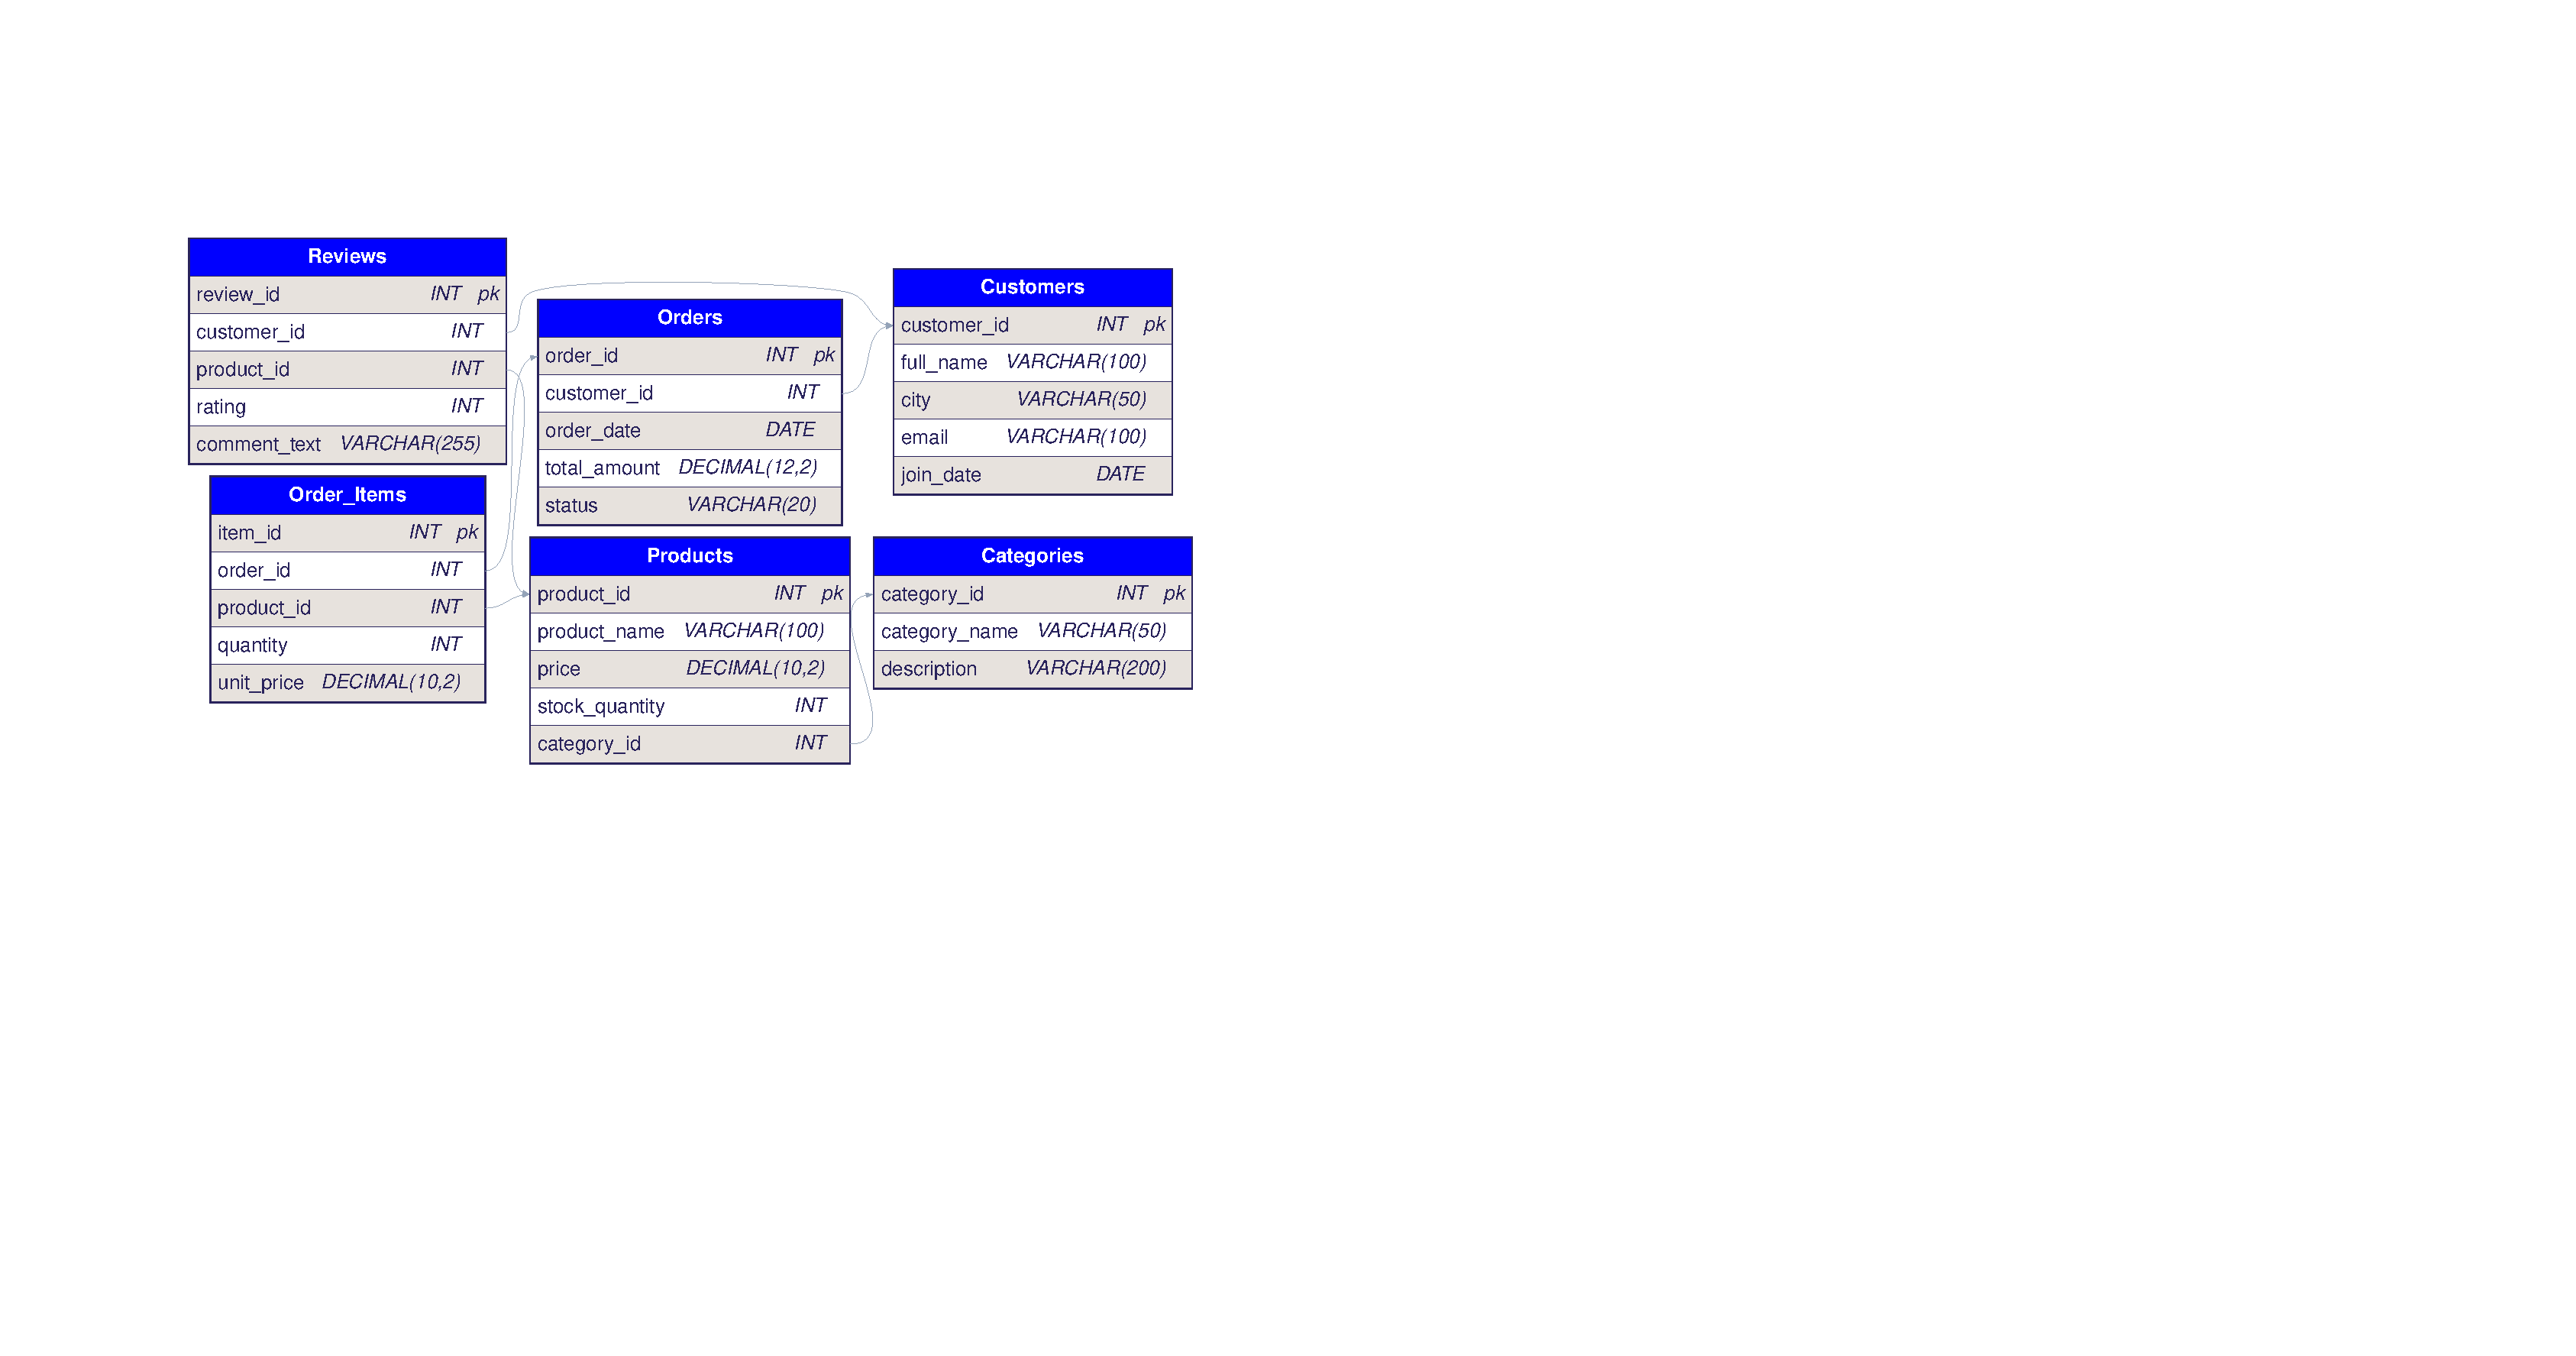
\includegraphics[trim={1cm 12cm 30cm 5cm}, clip, width=0.8\textwidth]{lab_04_schema.pdf}
    \end{figure}


\begin{enumerate}

    % ============================================================
    % Type 1: Sorting and Limiting Data (ORDER BY, LIMIT)
    % ============================================================

    \item Retrieve the names and prices of all products, sorted by price from highest to lowest.
    % Solution:
    % SELECT product_name, price 
    % FROM Products 
    % ORDER BY price DESC;

    \item List all customers sorted alphabetically by their full name.
    % Solution:
    % SELECT full_name, city 
    % FROM Customers 
    % ORDER BY full_name ASC;

    \item Find the top 5 most expensive orders placed based on \texttt{total\_amount}.
    % Solution:
    % SELECT order_id, total_amount 
    % FROM Orders 
    % ORDER BY total_amount DESC 
    % LIMIT 5;

    \item List the \texttt{product\_name} and \texttt{stock\_quantity} of products, sorted first by \texttt{category\_id} (ascending) and then by \texttt{stock\_quantity} (descending).
    % Solution:
    % SELECT product_name, category_id, stock_quantity 
    % FROM Products 
    % ORDER BY category_id ASC, stock_quantity DESC;

    \item Retrieve the 3 most recent orders (based on \texttt{order\_date}).
    % Solution:
    % SELECT order_id, order_date 
    % FROM Orders 
    % ORDER BY order_date DESC 
    % LIMIT 3;

    \item List all reviews sorted by rating (lowest first); if ratings are equal, sort by \texttt{review\_id} descending.
    % Solution:
    % SELECT review_id, rating, comment_text 
    % FROM Reviews 
    % ORDER BY rating ASC, review_id DESC;

    % ============================================================
    % Type 2: Range and Set Operators (BETWEEN, IN, DISTINCT)
    % ============================================================

    \item Find the names of products with a price between 50 and 200 (inclusive).
    % Solution:
    % SELECT product_name, price 
    % FROM Products 
    % WHERE price BETWEEN 50 AND 200;

    \item Retrieve unique city names where your customers reside.
    % Solution:
    % SELECT DISTINCT city 
    % FROM Customers;

    \item Find all orders placed between \texttt{'2023-06-01'} and \texttt{'2023-12-31'}.
    % Solution:
    % SELECT order_id, order_date, total_amount 
    % FROM Orders 
    % WHERE order_date BETWEEN '2023-06-01' AND '2023-12-31';

    \item List the names of customers who live in \texttt{'New York'}, \texttt{'Chicago'}, or \texttt{'Miami'}.
    % Solution:
    % SELECT full_name, city 
    % FROM Customers 
    % WHERE city IN ('New York', 'Chicago', 'Miami');

    \item Find products that belong to category IDs 1, 3, or 5 using the \texttt{IN} operator.
    % Solution:
    % SELECT product_name, category_id 
    % FROM Products 
    % WHERE category_id IN (1, 3, 5);

    \item Retrieve unique \texttt{product\_id}s that have received a review.
    % Solution:
    % SELECT DISTINCT product_id 
    % FROM Reviews;

    % ============================================================
    % Type 3: Single-Row Subqueries (Scalar Comparisons)
    % ============================================================

    \item Find the products that are more expensive than the average price of all products.
    % Solution:
    % SELECT product_name, price 
    % FROM Products 
    % WHERE price > (SELECT AVG(price) FROM Products);

    \item Retrieve the customer(s) who placed the specific order with the highest \texttt{total\_amount} in the database.
    % Solution:
    % SELECT full_name 
    % FROM Customers 
    % WHERE customer_id = (
    %     SELECT customer_id 
    %     FROM Orders 
    %     ORDER BY total_amount DESC 
    %     LIMIT 1
    % );

    \item List products that have less stock than the average stock quantity of all products.
    % Solution:
    % SELECT product_name, stock_quantity 
    % FROM Products 
    % WHERE stock_quantity < (SELECT AVG(stock_quantity) FROM Products);

    \item Find the name of the product that has the lowest price in the entire inventory.
    % Solution:
    % SELECT product_name 
    % FROM Products 
    % WHERE price = (SELECT MIN(price) FROM Products);

    \item Find orders where the \texttt{total\_amount} is greater than the average total amount of all orders.
    % Solution:
    % SELECT order_id, total_amount 
    % FROM Orders 
    % WHERE total_amount > (SELECT AVG(total_amount) FROM Orders);

    \item Retrieve the name of the customer who has the earliest \texttt{join\_date} (i.e., the first customer to join).
    % Solution:
    % SELECT full_name, join_date 
    % FROM Customers 
    % WHERE join_date = (SELECT MIN(join_date) FROM Customers);

    % ============================================================
    % Type 4: Nested/Multi-Row Subqueries (IN, Nested Logic)
    % ============================================================

    \item Find the names of products that belong to the \texttt{'Furniture'} category (using a subquery on the \texttt{Categories} table).
    % Solution:
    % SELECT product_name 
    % FROM Products 
    % WHERE category_id = (
    %     SELECT category_id 
    %     FROM Categories 
    %     WHERE category_name = 'Furniture'
    % );

    \item Find the full names of customers who have placed at least one order (check if \texttt{customer\_id} is in the \texttt{Orders} table).
    % Solution:
    % SELECT full_name 
    % FROM Customers 
    % WHERE customer_id IN (SELECT customer_id FROM Orders);

    \item Find the names of products that have \textbf{never} been ordered (product ID not in \texttt{Order\_Items}).
    % Solution:
    % SELECT product_name 
    % FROM Products 
    % WHERE product_id NOT IN (SELECT product_id FROM Order_Items);

    \item \textbf{Deep Nesting:} Find the names of customers who have ordered a product from the \texttt{'Smartphones'} category.
    % Solution:
    % SELECT full_name 
    % FROM Customers 
    % WHERE customer_id IN (
    %     SELECT customer_id 
    %     FROM Orders 
    %     WHERE order_id IN (
    %         SELECT order_id 
    %         FROM Order_Items 
    %         WHERE product_id IN (
    %             SELECT product_id 
    %             FROM Products 
    %             WHERE category_id = (
    %                 SELECT category_id 
    %                 FROM Categories 
    %                 WHERE category_name = 'Smartphones'
    %             )
    %         )
    %     )
    % );

    \item Find the \texttt{review\_id} and \texttt{comment\_text} for reviews written by customers from \texttt{'New York'}.
    % Solution:
    % SELECT review_id, comment_text 
    % FROM Reviews 
    % WHERE customer_id IN (
    %     SELECT customer_id 
    %     FROM Customers 
    %     WHERE city = 'New York'
    % );

    \item Find products that have been ordered in a quantity greater than 2 in a single line item (using \texttt{Order\_Items}).
    % Solution:
    % SELECT product_name 
    % FROM Products 
    % WHERE product_id IN (
    %     SELECT product_id 
    %     FROM Order_Items 
    %     WHERE quantity > 2
    % );
    % ============================================================
    % Type 5: Correlated Subqueries & Advanced Logic
    % ============================================================

    \item Find products that are more expensive than the average price \textbf{of their specific category}.
    % Solution:
    % SELECT p1.product_name, p1.price, p1.category_id
    % FROM Products p1
    % WHERE p1.price > (
    %     SELECT AVG(p2.price) 
    %     FROM Products p2 
    %     WHERE p2.category_id = p1.category_id
    % );

    \item \textbf{Correlated:} Find customers who have placed an order but have \textbf{never} written a review.
    % Solution:
    % SELECT full_name 
    % FROM Customers c
    % WHERE customer_id IN (SELECT customer_id FROM Orders)
    % AND customer_id NOT IN (SELECT customer_id FROM Reviews);

    % \item Find the category name that contains the product with the highest price.
    % Solution:
    % SELECT category_name 
    % FROM Categories 
    % WHERE category_id = (
    %     SELECT category_id 
    %     FROM Products 
    %     WHERE price = (SELECT MAX(price) FROM Products)
    % );

    \item Find customers who have ordered the product named \texttt{'Dell XPS 13'}.
    % Solution:
    % SELECT full_name 
    % FROM Customers 
    % WHERE customer_id IN (
    %     SELECT customer_id 
    %     FROM Orders 
    %     WHERE order_id IN (
    %         SELECT order_id 
    %         FROM Order_Items 
    %         WHERE product_id = (
    %             SELECT product_id 
    %             FROM Products 
    %             WHERE product_name = 'Dell XPS 13'
    %         )
    %     )
    % );

    \item Find products that have a rating lower than the average rating of all reviews.
    % Solution:
    % SELECT product_name 
    % FROM Products 
    % WHERE product_id IN (
    %     SELECT product_id 
    %     FROM Reviews 
    %     WHERE rating < (SELECT AVG(rating) FROM Reviews)
    % );

    \item \textbf{Correlated:} Find orders where the \texttt{total\_amount} is larger than the average total amount of orders placed by that specific customer.
    % Solution:
    % SELECT o1.order_id, o1.customer_id, o1.total_amount
    % FROM Orders o1
    % WHERE o1.total_amount > (
    %     SELECT AVG(o2.total_amount)
    %     FROM Orders o2
    %     WHERE o2.customer_id = o1.customer_id
    % );

\end{enumerate}
\end{document}